\section{Algorithm Design}
In this section, we will elaborate on the design of our algorithm, and our rationale behind our design choices,
as well as the our procedures and results and brought us to our conclusions.

\subsection{Overview}
Figure \ref{fig:algoOverview} shows the information flow through our core algorithm. This core
algorithm is responsible for taking in images, and returning the text present in the image.
	\begin{figure}[h]
		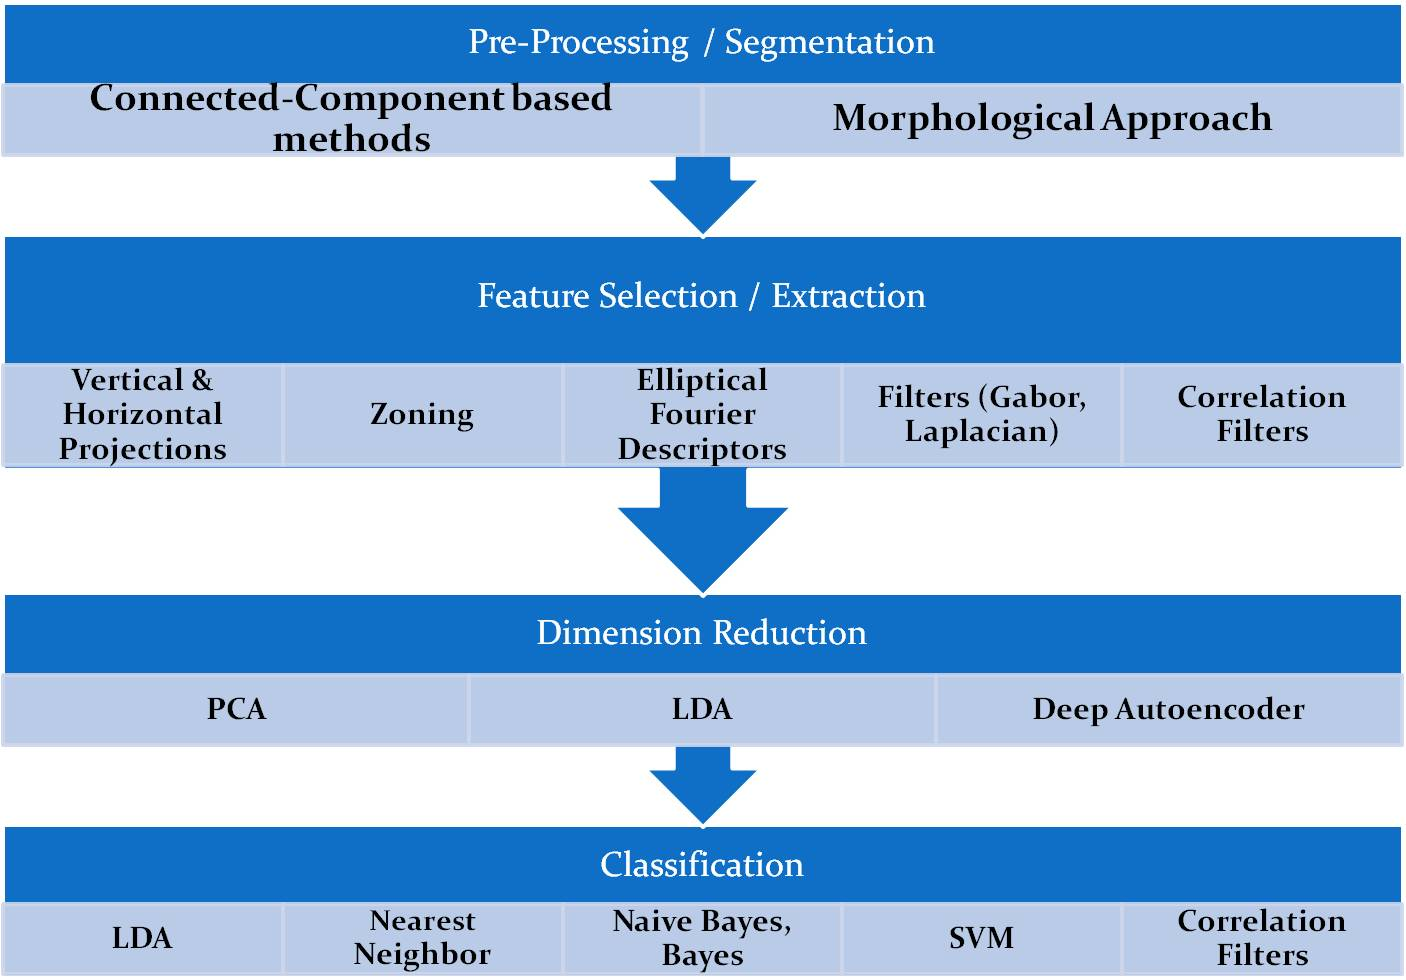
\includegraphics[scale=0.66]{algoOverview.jpg}\\
		%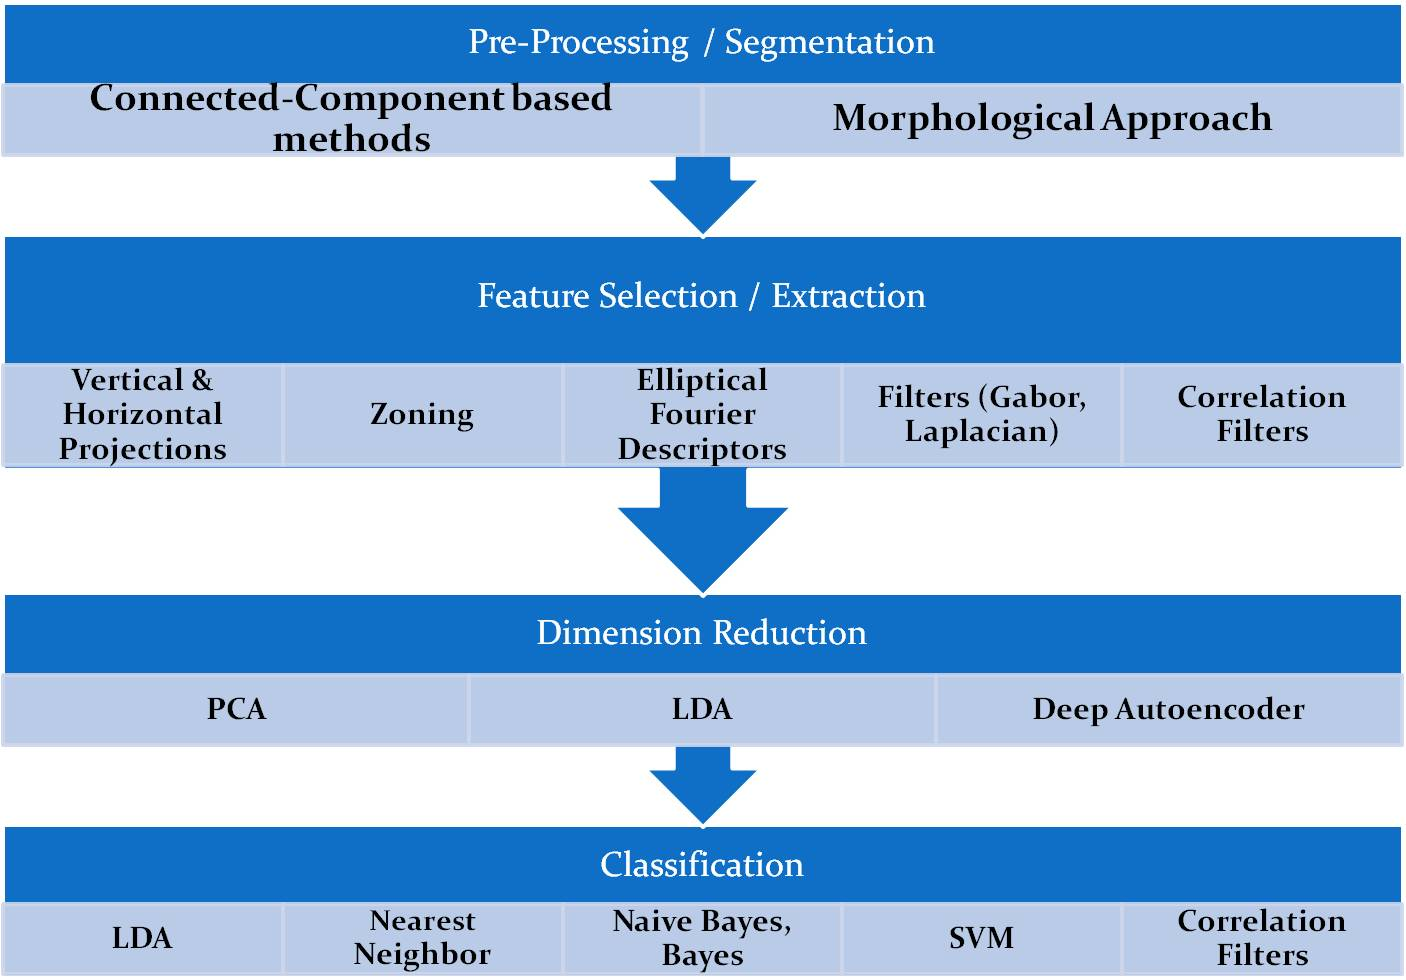
\includegraphics[height=90mm, width=170mm]{algoOverview.jpg}\\
		\caption{Information flow through Core Algorithm}
		\label{fig:algoOverview}
	\end{figure}
As can be seen, we broke up our core algorithm into four main components: Pre-Processing / Segmentation,
Feature Selection / Extraction, Dimension Reduction and Classification. This approach had been used by other teams
also implementing OCR previously \cite{tai, zhidong, sonia}, and we decided to use it based on its simplicity and modularity.\\





\subsection{Principal Considerations}
Due to the nature of our project, we were constrained by both time (~6 weeks), as well as resources (limited number of approaches
to try, platform specifications). Our core considerations, too, in choosing algorithms were:\\

\paragraph{\textit{Simple to implement}} Given our short time frame, we were looking for algorithms that would be simple to implement, and
quick to debug. Simple algorithms would also there was a greater chance of successfully porting it over from MATLAB to Java to C,
or in some cases a built in function might already exist.

\paragraph{\textit{Modular}} Our project had been set up to be modular, with different components being able interchangeable. This allowed us
to quickly experiment with different algorithmic components and gauge the accuracy of that model. Naturally, it was much more beneficial if
the algorithm was modular to fit into our development framework.

\paragraph{\textit{Memory Efficient}} The Android platform does not provide large amounts of memory to its applications. Given that we were
also dealing with large bitmaps sometimes, it was crucial to have a memory efficient algorithm to prevent Out of Memory Errors.

\paragraph{\textit{Fast, Minimum Computation}} We wanted our algorithms to run quickly, and efficiently. In the long run, we hoped to scale
up such that we could work on live data.
\paragraph{\textit{Robustness}} We wanted our OCR engine to be robust to noise, and having algorithms that gracefully deal with this would
be a plus.\\

We then used these considerations as a metric in choosing which algorithms to include into our project. As a benchmark, all testing
of the algorithms in this section was done with the same dataset: Numbers 0-9, Binary images of varying font and rotation. Training
was done on 50 samples, and testing was done on 20 samples, of each number. Figure \ref{fig:sampleData} are some examples of the characters from the training dataset.\\
\begin{figure}[h]
		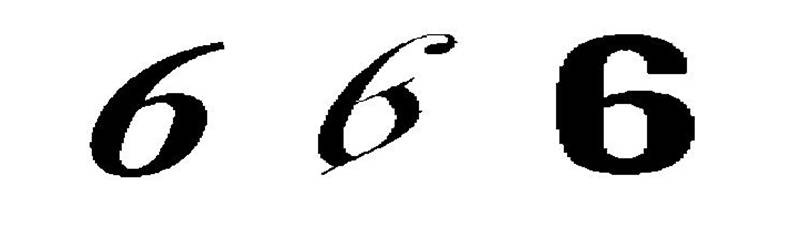
\includegraphics{sampleData.jpg}\\
		\caption{Sample of Training Dataset used. Binary images of varying font, and rotation.}
		\label{fig:sampleData}
\end{figure}





\subsection{Pre-Processing / Segmentation}
When choosing components, we first decided on Pre-Processing / Segmentation, as it was the initial step before any computation, and would define
the format of the data we would be training on. We initially experimented with connected component based methods \cite{textDetectionSurvey, ohya},
whereby we would be applying local thresholding for binarization, and detecting blobs of similarly textured grayscale as objects. Essentially,
we were using the gray-level difference of shapes and sizes to make a match. We found it worked relatively well, but was susceptible to noise
and illuminating conditions. Subsequently, we tried another approach. This time we implemented a morphological approach \cite{hassan}, essentially
doing edge detection. We would form a weighted grayscale and identify the edges using a morphological gradient operator. Use of dilation and erosion
allowed us to remove salt and pepper noise, as well as form candidate regions for segmentation. We also found that using adaptive thresholding worked
best for the binary edge image. The algorithm became much more robust to noise and orientation, but was still suscpetible to illumniation, as shown
in the picture below. This was chosen as our segmentation algorithm for the project
\begin{figure}[h]
		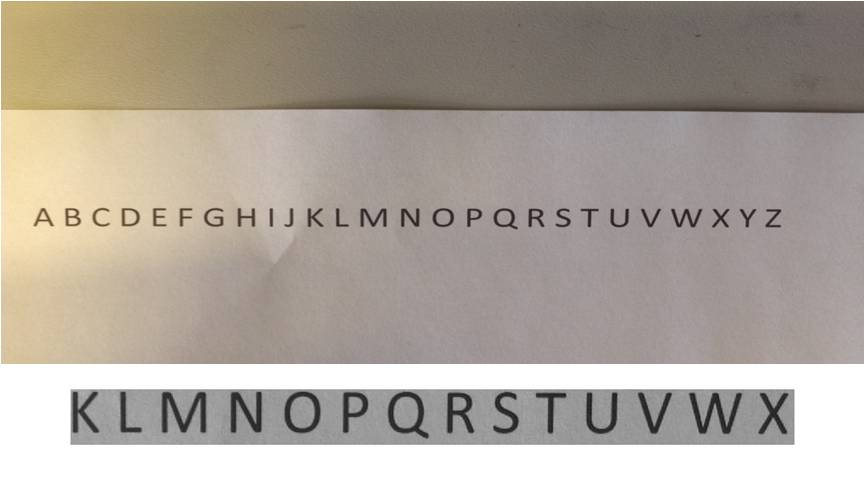
\includegraphics{seg.jpg}\\
		\caption{Morpohlogical Image Segmentation with Strong illumination from left, Above: Image, Below: Detected text}
		\label{fig:seg}
\end{figure}





\subsection{Dimension Reduction}
We next turn our attention to Dimension Reduction. Dimension Reduction tends to have some overlap with feature selection and extraction, but
we decided to seperate it out, to keep our project modular. Dimension Reduction was meant to ensure that the inputs of the feature vector to 
the classifier would be uncorrelated, and that the dimensions would be reduced to a set number. The idea was to decrease computational complexity
of the classification algorithm when training, by using a smaller feature vector that still captured the majority of variance in the dataset.

\subsubsection{Linear Discriminant Analysis}
Linear Discriminant Analysis attempts to model the difference between the classes of data, by taking into account class labels and maximizing the
between-class scatter under the constraint that the within-class scatter is minimized. This results in compact clusters for each class, as far as
possible from each other. To test LDA, we attempted to reconstruct a test image, and measure the mean squared error compared to the original image.
LDA performed well, with almost no reconstruction error.
\subsubsection{Autoencoder}
\begin{figure}[h]
		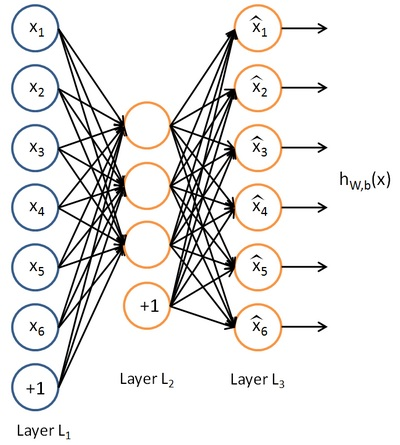
\includegraphics[scale=0.75]{autoencoder.jpg}\\
		\caption{Structure of an autoencoder. Implements Nonlinear PCA by attempting to learn the function $h_{W,b}(x) \approx x$}
		\label{fig:autoencoder}
\end{figure}
Autoencoders are essentially a way of implementing Nonlinear PCA. This is done using a neural network applying backpropagation, where the
hidden layers are used to provide a nonlinear reconstruction. In order to train it, we set the target values to be equal to the inputs, such
that the network attempts to learn an approximation of the identity function, so that the output is similar to the input. By varying the number 
of output nodes (number of nodes in Layer $L_3$,
we can select the number of basis function to use (similar to PCA in how we can choose how many eigenvectors to use). As such, since the number
of hidden units is much less that the input feature vector, Layer $L_1$, the network learns a compressed representation of the input. By imposing
a sparsity constraint on the network, as well as implementing a locally competitive algorithm, could potentially provide us better, more meaningful
representations too. Varying the number of hidden layers also affects the output - multiple sigmoid hidden layers give us our nonlinear representation.
For our project, we tested the autoencoder to see if there was significant benefit using a non-linear approach. We ran the data through a 5-layer 
autoencoder. The representation we got out did not significantly improve beyond PCA.

\subsubsection{Principal Component Analysis}
PCA performed well, and is typically the most basic dimension reduction method to use. For our purposes, we found the reconstruction error to be
~1\% or less, similar to LDA.\\

After our testing, we decided to utilize PCA, due to its simplicity and modularity. It also had inbuilt functions in OpenCV and Matlab, allowing
it to be quickly implemented. The autoencoder might have performed well after additional research (We only tested it thrice), but given the time
constraints, and seeing that it did not bring significant immediate benefit, plus we would essentially have to write the neural network on Android ourselves,
made us decide on using PCA.



\subsection{Feature Selection / Extraction}
In OCR, feature selection is key, and is closely tied to classification. For this section, we will
be decribing some of the features we opted to use \cite{line, jain}. The analysis of their effectiveness is in the Results section.

\subsubsection{Vertical \& Horizontal Projections}
\begin{figure}[!]
		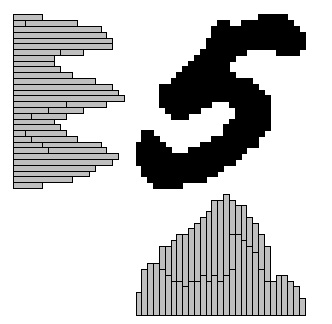
\includegraphics[scale=0.33]{proj.jpg}\\
		\caption{Diagram showing Vertical and Horizontal Projections}
		\label{fig:proj}
\end{figure}
Figure \ref{fig:proj} shows the vertical and horizontal projection feature. Essentially, it is taking a spatial
histogram of the number of black pixels row by row, and column by column. The feature vector is then the concatenation
of both histogram values. Initial results showed this feature having a \~60\% accuracy on the test dataset mentioned above.
This has the advantage of being simple, and
quick to compute. However, it is susceptible to rotation, as a rotation would shift both histograms by some amount.
In addition, it is also susceptible to illumination. Being in a shadow tends to increase the number of black pixels
shown, and hence will distort the feature vector. In order to test its effectiveness, we varied the number of bins,
to account for some rotation. We also equalized the histogram, and normalized the feature vector. However, these
did not significantly improve the accuracy.\\

\subsubsection{Zoning}
\begin{figure}[!]
		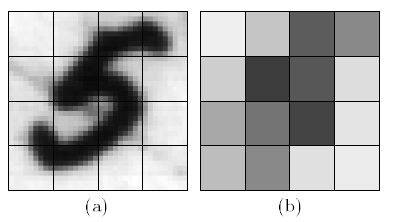
\includegraphics[scale=0.25]{zone.jpg}\\
		\caption{Diagram showing Zoning of Characters: a) Bitmap of Character b) Feature Vector formed}
		\label{fig:zone}
\end{figure}
Figure \ref{fig:zone} Shows how the feature vector is computed during zoning. The rectangle circumscribing the character 
is divided into several overlapping, or nonoverlapping, regions and the densities of black points within these regions are computed
and used as features. Initial results showed this feature also having a \~60\% accuracy on the test dataset mentioned above. Again, this has the advantage of being simple, and
quick to compute. However, it is slightly susceptible to rotation.
In addition, it is also susceptible to illumination. Varying the number of zones, and their overlaps did not. significantly improve the accuracy.\\


\subsubsection{Elliptical Fourier Descriptors}
\begin{figure}[h]
		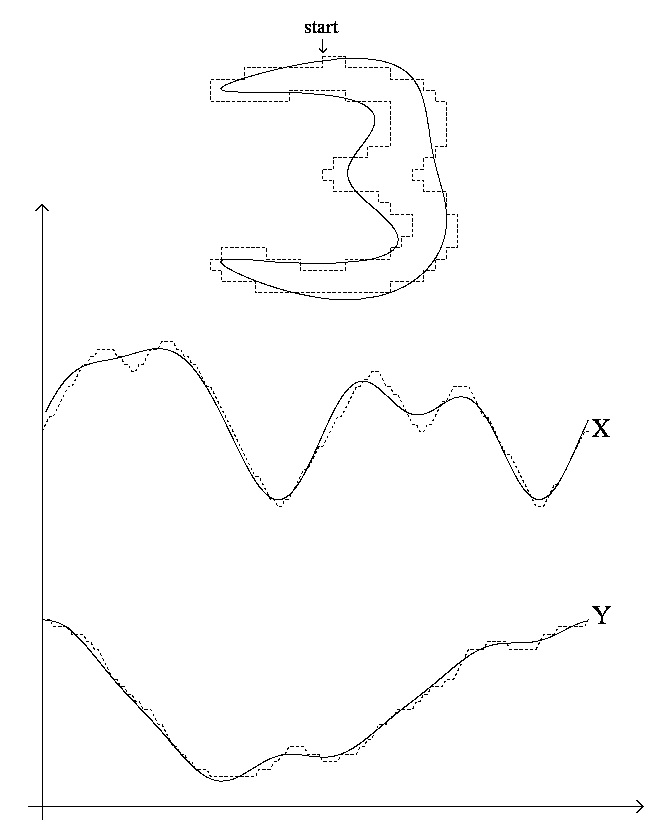
\includegraphics[scale=0.5]{elliptical1.jpg}\\
		\caption{Diagram showing Zoning of Characters}
		\label{fig:elliptical1}
\end{figure}
Figure \ref{fig:elliptical1} shows the construction of the curves from the contours.
The closed outer contour curve of a character is a closed piecewise linear curve that passes through the centers of all the pixels which
are 4-connected to the outside background, and no other pixels. This is because we are only using numbers and upper-case alphabets. Following the
curve, the pixels can be visited in counter-clockwise order, and the curve may visit an edge pixel twice at locations where the object is one-pixel wide.
As such, the contour is made up of line segments, each a straight line between the pixel centers of two 8-connected neighbors. By approximating the
contour curve by a parametric expression, the coefficients of the approximation can be used as features. By following the close contour successively,
a periodic function results, which are well suited to Fourier series expansion. This requires an arbitary stating point to be chosen. To mitigate this,
we calculate the phase shift from the first major axis, and rotate the coefficients to achieve a zero phase shift. For rotational invariant descriptors, the rotation
of the semi-major axis is found and descriptors are rotated once more. Size invariance is achieved by dividing by the magnitude of the semi-major axis.
Elliptical Fourier Descriptors are used to reduce the dimensionality of the feature vector and the extract features made invariant to global deformations
such as translation and rotation.

\begin{figure}[h]
		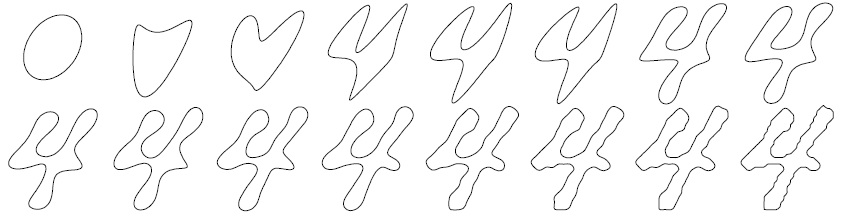
\includegraphics[scale=0.75]{elliptical.jpg}\\
		\caption{Character '4' reconstructed by elliptic Fourier descriptors of orders up to 1, 2, ... 10; 15, 20, 30, 40,  50, and 100 respectively}
		\label{fig:elliptical}
\end{figure}
Figure \ref{fig:elliptical1} shows the reconstruction of the character using elliptic fourier descriptors. As additional terms are added, the accuracy of
the curve increases. This feature take longer to compute, however, it is both rotational and size invariant. We are also able to choose the number
of 'harmonics' we would like to use, therefore giving us flexibility in choosing our feature vector. The initial implementation of the elliptical fourier
descriptor was written by us, however, later version referenced online sources.

\subsubsection{Filter (Gabor, Laplacian)}
We utilized both the Laplacian and Gabor filters in our filter bank. Both filters are useful as spatial edge detectors, and produced
good results when we initialized our Gabor filter bank with different frequencies and orientations. As we learned in the homework, this produced
good features for discrimination. However, our feature vector was extremely large, and slow to compute due to the numerous computations and convolutions.

\subsubsection{Correlation Filters}
The correlation filters will be elaborated in greater detail in the results section.



\subsection{Classification}
In choosing our classification method, we decided to take two different approaches to implement the OCR engine. We wanted
to try both the feature matching and template matching approaches, and as such chose to use SVMs and Correlation Filters in the final product.

\subsubsection{Linear Discriminant Analysis}
LDA performed well in classification, with an accuracy of \~95\%. This is probably as the disciminatory information was in the mean of the data.
However, it did not bear itself well to implementation on the Android platform, and produced a hard bound of at most number of classes -1 feature
projections. When scaling up to the full alphabet, it did not seem likely continue to be modular on the Android platform. As such, we decided not
to proceed with using LDA.

\subsubsection{Nearest Neighbor}
Nearest neighbor is a simple classifier that is based on the nearest-neighbor approach. For classification, one simply finds the N-dimensional 
feature space the closest character from the trainng set to an character being classified. if the neighbor is nearby, it is likely to be similar to 
the character being classified and so can be grouped as such. It is simple to implement, can be generalized to k-means, and worked reasonably 
well for small datasets (\~85\% accuracy). However, when increasing the number of classes, as well as the necessary training data, we found 
that accuracy decreased significantly. Choosing parameters was also tricky, in that it seemed sensitive to the presence of irrelevant parameters.
In addition, the training set is retained in its entirety as a description of the character distribution,
and with our current memory constraints on Android, it did not seem particularly fruitful. 

\subsubsection{Naive Bayes}
The Naive Bayes classifier was fast to train and evaluate, and seemed to perform well quickly on small datasets (5 characters, 50 training samples),
with an accuracy of \~95\%. However, when scaling up the number of classes the algorithm did not seem to be able to solve the harder classification
problems with the same amount of accuracy. Naturally, the algorithm assumes that the features are independent, which is probably not true given our
data. As such, we decided to not to pursue Naive Bayes in our implementation.

\subsubsection{Support Vector Machine}
Support Vector Machines are powerful non-linear classifier that gave us great potential for an OCR engine, given that we could
have good features. While they were slow to train, they consistent produced good results (\~99\% accuracy with 10 classes). In addition,
by increasing the dimensionality of the data, the characters get easier to separate, allowing it to solve classification problems with
arbitarry complexity. Using the dot product, and the model's support vectors (there is no need to store all the points in an SVM), with biases,
we thought it would be possible to move a trained SVM onto the android platform, with less of a memory footprint than expected. As such, it seemed
that given the great potential, the only risk would be bad features and a long training schedule. We later mitigated this by training our
SVMs on the ECE Servers over command line - with 8 Cores running lots of RAM, we could train our entire dataset of 25200 characters in 2 hours.

\subsubsection{Correlation Filters}
The correlation filters will be elaborated in greater detail in the results section.
